
\section{Magnitude Estimation For System-Level Evaluation}
\label{sec:rq2}

The third research question RQ\ref{item:rq2} concerns the direct
application of magnitude estimation relevance judgments for the
evaluation of IR systems, by considering their use for calibrating
gain levels in two most widely-used gain-based IR evaluation metrics, nDCG
and ERR.

% \sm{should we add some other metric? That Graded-MAP mentioned by
%   referees?} 
%   \fs{My vote is no. I have never seen ``graded MAP'' used for anything,
%   anywhere... so who cares? :-)}
%   \aht{ok, no.}

\subsection{Gain in the nDCG and ERR Metrics}
\label{sec:ndcg-err}

Magnitude estimation provides scores
that reflect ratios of human perceptions of the intensity 
of relevance of
different documents in relation to a topic.
This is directly related to the notion of gain in effectiveness metrics
such as normalized discounted cumulative gain (nDCG).
For example, 
\citet{JarKek02} describe ``cumulative relevance gain'' that a user
receives by examining a search results list, and discuss setting
``relevance weights at different relevance levels''.
That is, weights are applied to each level of an ordinal relevance scale,
and can be chosen to reflect different assumptions about searcher
relevance behavior.
However, the ``standard'' approach that has been adopted when using nDCG
is to simply assign ascending integer values to the ordinal levels,
starting with 0 for the lowest (non-relevant) level; for a 3-level
ordinal scale, the default gains would be 0, 1 and 2, as for example
implemented in {\tt
trec\_eval}.\footnote{\url{http://trec.nist.gov/trec_eval}}

In addition to modeling different levels of gain, or relevance,
the discounted cumulative gain metric also includes a discounting
function, 
so that documents that are retrieved further down in a ranked search
results list contribute smaller amounts of gain, reflective of 
factors such as the effort or time that a user must invest while working
their way through the list~\cite{JarKek02}.
Using a logarithmic discount, discounted cumulative gain
at cutoff N is calculated as 
\[
\mathrm{DCG@N} = G_1 + \sum^{N}_{i=2} \frac{G_i}{\log_2(i)},
\]
\noindent where $G_i$ is the gain value for the document at position $i$
in the ranked list. To enable fair comparisons
across topics with different numbers of relevant documents, the DCG@N
score is divided by an \emph{ideal} gain vector, a
ranking of documents in decreasing relevance order, to obtain normalized
discounted cumulative gain, nDCG@N.

Expected reciprocal rank is 
a
metric based on a cascade
model of searcher behavior, where the probability of continuing on to
the next position in the ranked results list is influenced by the
relevance of previous items. The metric calculates the expected
reciprocal rank at which the searcher will stop~\citep{ChaMet09}, and is defined
as
\[
  \mathrm{ ERR@N} = \sum^{N}_{i=1} \frac{R(G_i)}{i} \prod^{i-1}_{j=1}(1 - R(G_i)),
\]
\noindent where $R(G) = (2^{G_i}-1) / 2^{\max(G_i)}$. 
In the analysis that follows, we calculate both nDCG and ERR
up to a depth of $N=10$.

For both nDCG and ERR, gain is based on the relevance of a document,
which has previously been measured on an ordinal scale, typically with
3~\cite{KanAsl03} or 4~\cite{JarKek02} levels, depending on the test
collection being used.
Since magnitude estimation relevance judgments are continuous rather
than ordinal in nature, and reflect the perceived level of relevance
for individual topic-document combinations, it is possible to assign
more fine-grained gain values, potentially reflecting different gains
for individual documents, or even for individual searchers.

\subsection{Comparative System Rankings}
\label{sec:ranking-trec-runs}

Given that the agreement between our magnitude scores, TREC judgments
and Sormunen's judgments is not perfect, it is reasonable to expect
that relative system effectiveness orderings computed with each of
these as a basis may differ.
We first examine the correlation between system orderings using
magnitude estimation scores and TREC relevance as gain values, as for
both these judgment sets we have nearly complete coverage of the top 10
documents of all runs submitted to TREC-8, for our 18 judged topics.
% In the conference version of this paper~\cite{ME-SIGIR15} we showed the
% system scores (mean over all 18 topics) using median magnitude
% estimation scores per document (x-axis), and binary TREC categories
% (y-axis).
% This gave a result similar to Figure~\ref{fig:runs-rerank-median3best}.
% Unjudged documents were assumed to be irrelevant, as is common practice
% when using TREC data.
% \aht{What do you think of this almost self-referential style?}
% 
% Here we make a small alteration to the aggregation of the ME scores to
% get a single score for a document.
Rather than taking the median of all scores assigned to a document, we
take the median of scores taken from the three units that have document
orderings that have the highest agreement with the TREC orderings, or
Sormunen orderings, respectively.
In effect, the scores derived from units with high internal agreement as
computed in Section~\ref{sec:internal-agreement}, with ties broken in favor
of units with the least unjudged documents.
By aggregating scores over units that have a high agreement with the
original TREC orderings, any differences in system rankings we see should be more
attributable to the scale of the gain values, rather than perturbations in
document orderings given by different gain values.
\textcolor{red}{Note that this is a slightly less confounded methodology 
than was used in our previous paper~\cite{ME-SIGIR15}, which simply took the median 
of all units, even if the unit wildly disagreed with the ordering of documents
given by the categorical judgments. This revised methodology accounts for the 
differences between the figures and tables in this section and 
in the previous paper.}

Figure~\ref{fig:runs-rerank-median3best} shows the concordance between
system rankings using TREC categories and ME scores as gain values.
It can be seen that there are definite changes in system rankings when
using the different relevance scales, with Kendall's $\tau$
correlations of 0.677 and 0.222 for nDCG@10 and ERR@10, respectively.
As the aim of system evaluation is to identify top-performing systems,
we also consider changes in the \emph{top set}, defined as the group of
systems that are statistically indistinguishable from the system with
the highest mean effectiveness, using a paired Wilcoxon signed-rank
test with $p<0.05$.
These systems are shown as red dots.
The overlap of the top set, based on the TREC and magnitude estimation
relevance judgments is 82\% for nDCG@10 and 20\% for ERR@10, confirming
that the perturbation in system ordering has an impact on which systems
are identified as being the best performers.

Since the Sormunen judgments only cover around 19\% of the documents
that occur in the top 10 of all TREC-8 ad hoc runs, evaluating the
original runs using these relevance judgments is problematic, due to
the large number of unjudged documents.
However, the judgment coverage of individual ranked lists (that is,
for particular topics within a run) varies substantially.
Therefore, to enable a comparison between the ordinal judgment and
magnitude estimation judgments on system orderings, we simulate 
runs that only include ranked lists for topics that are fully judged by
Sormunen.

For each topic, we identify all ranked lists within the full
set of runs that have Sormunen judgments for all top 10 documents for
that topic; we call each of these a 
\emph{complete sub-run}.
There are 12 topics where there are at least two complete sub-runs out of
all of the TREC-8 ad hoc runs for that topic.
To form a simulated retrieval system, we then randomly choose one
complete sub-run for each of the 12 topics to
give a ``full run'' over all 12 topics.
Using this method, we construct 100 simulated system runs that are
random merges of complete sub-runs from real 
runs.
While these simulated systems are not actual TREC submissions, they are
plausible in that each individual topic ranking is from a real TREC
run.

Figure~\ref{fig:runs-rerank-median3best-fake} shows that there is also a
large discordance between the system rankings using the Sormunen
categories and magnitudes as gain values.
However, note that the scale is different in this figure than in
Figure~\ref{fig:runs-rerank-median3best}, as the simulated systems all have
relevant documents in the top 10, and so are high scoring.
Correlation as measured by Kendall's $\tau$ is even lower here, at 0.147
and 0.06 for nDCG@10 and ERR@10, respectively.
The overlaps in top sets are 32\% for nDCG@10 and 68\% for ERR@10.
The relatively high performance of systems on this simulated collection
is to be expected, as only complete sub-runs were selected, and around
half of the Sormunen judgments are for documents that were originally
rated as relevant by TREC, and so the runs in the simulated systems
have a high number of relevant documents.
It is interesting that there is still a sizable change in the top
set using either metric with the different judgments, however.

\subsection{Judgment Variability and System Rankings} 
\label{sec-judge}
%%%
%%%\sm{we should be consistent: there is a consistent variability or not?
%%%  Can it be ascribed only at individual relevance perceptions?}
%%%\sm{we should be consistent also in terminology:   ``disagreement'',
%%%  not ``variability''?} 
%%%\fs{Completely agree that we need to be careful with terminology and use
%%%it consistently. However, i think these two things are actually quite
%%%different: agreement is some measure of how well-aligned judgements are
%%%(e.g. percent of consistent pairwise ordering); variability is the
%%%differences in actual assigned ME scores as a 
%%%reflection of different perceptions of relevance?}
%%%\sm{ok, I buy this, need to write it down properly}
%%%
%%%\sm{As we have seen in Section~\ref{sec:judge-agreement} the agreement
%%%  is not perfect... 
%%%  quality is good, though, ... 
%%%  this can be ascribed to variability...}


%%%\sm{I've been thinking and rethinking over this. Some remarks:
%%%  \begin{itemize}
%%%  \item I think we felt short with this analysis. 
%%%    By selecting individual judges we sort of lose the benefit of the
%%%    crowd: it is rather accepted, if not well known, that
%%%    \emph{redundant} judgments need to be collected, in any
%%%    situation.  So in place of using individual scores I'd prefer to
%%%    use the median score of a proper subset of all 10 workers. 
%%%    (I'm not sure it will make a difference since we're taking several
%%%    samples, but still I guess it will be different)
%%%  \item Another reason for the low tau correlations below could be
%%%    that individual workers did not simply disagree on the magnitudes
%%%    and the scales, but also on the ranking. 
%%%    But we're neglecting this.
%%%    A better, or at least alternative, way of doing these experiments
%%%    would be to select only the workers that have a pairwise agreement
%%%    high enough with the ``official'' judges, so that any disagreement
%%%    can truly be ascribed to different scales. 
%%%    This is consistent with what Falk wrote in his last note above: we
%%%    select the workers with high pairwise agreement and we investigate
%%%    their variability.
%%%  \item All this needs to be re-thought after the results of
%%%    Section~\ref{sec:how-many-workers}. 
%%%  \item So in summary: take Section~\ref{sec:how-many-workers};
%%%    consider worker subsets rather than individual workers; select
%%%    only the workers with pairwise agreement high enough. Hm?
%%%  \end{itemize}
%%%  \aht{OK, i agree there is a confound that and this can be improved.
%%%I think we leave 6.3 out of this paper, and that makes this section 
%%%easier too. I will do (14 Dec).}
%%%}


\begin{figure}[tbp]
  \centering
  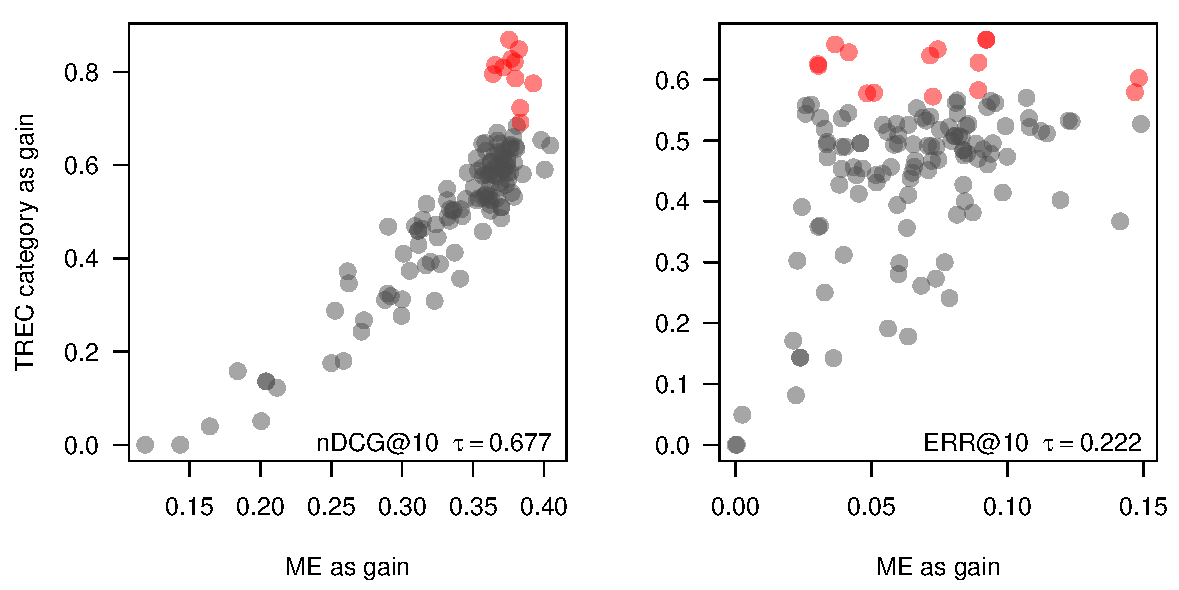
\includegraphics[width=.6\linewidth]{figs/sysRank_scatter_TREC_med3bestME.pdf}
  \caption{System scores using TREC categories (y-axis) 
    and magnitudes (x-axis) as gains in 
    the nDCG@10 and ERR@10 metrics. There is one dot for each of the 129 systems 
    participating in the TREC-8 ad hoc track, with red dots showing the top-set (see text).
    Magnitudes used are the median of the three units per document that most agree with TREC
    document rankings.
    Kendall's $\tau$ is shown. 
  \label{fig:runs-rerank-median3best}
  }
\end{figure}
\begin{figure}[tbp]
  \centering
  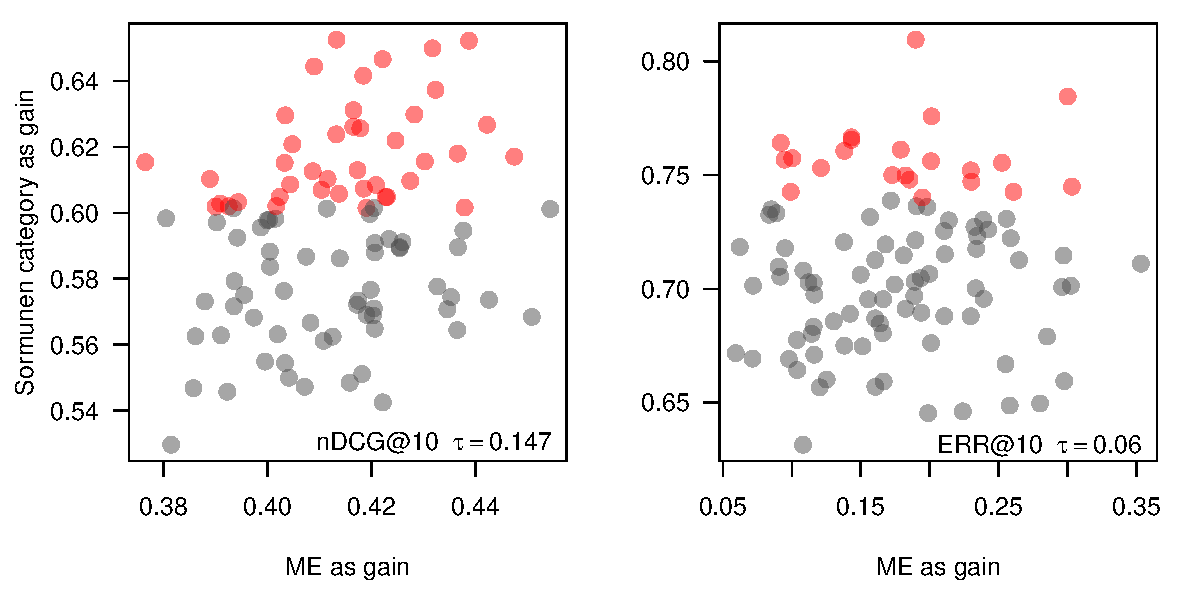
\includegraphics[width=.6\linewidth]{figs/sysRank_scatter_FAKE_medME3bestME.pdf}
  \caption{As for Figure~\ref{fig:runs-rerank-median3best} but using 
           Sormunen categories (y-axis) and simulated runs as described in the text.
  \label{fig:runs-rerank-median3best-fake}
  }
\end{figure}


The previous section showed that using magnitudes as gain led to
changes in the ranking of systems using different metrics, even when
only aggregating over magnitude judgments that agreed with individual pairwise
document rankings of the original categorical scale.
There is, however, substantial variation in the magnitudes assigned to documents
by our judges.
Perhaps using magnitudes from different judges would lead to different 
system rankings. 
As we have at least 10 judgments per topic-document pair, we can
re-sample individual scores many times, recompute system orderings, and
get a distribution of $\tau$ values.
The results are shown in Figure~\ref{fig:runs-rerank-resample}: the
correlations between system orderings seen in the previous section sit about in the middle 
of these distributions.
The spread of the distributions reflect the wide range of individual variation -- differences in
perceptions of relevance -- that in turn leads to a wide range of
$\tau$ values.
% \aht{I don't think I need to alter this as the median-of-best-3 aggregator falls withint he
% boxes.}

\begin{figure}[tbp]
  \centering
  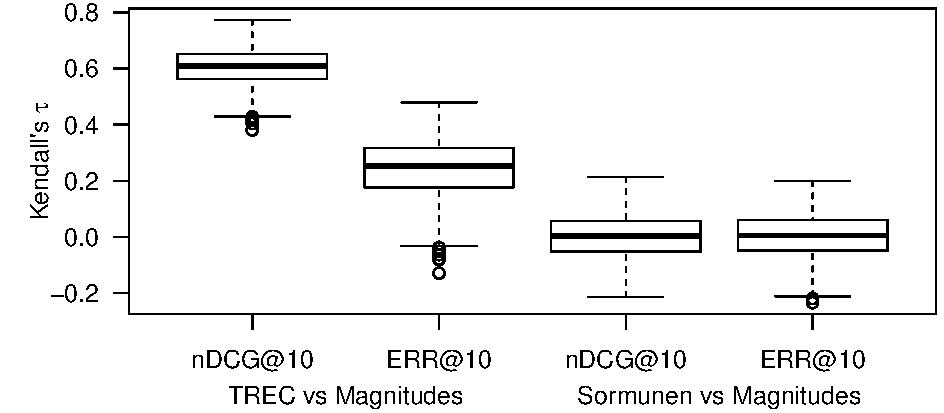
\includegraphics[width=.7\linewidth]{figs/metrics_resample.pdf}
  \caption{Kendall's $\tau$ between system rankings obtained using gains from 
    the judgments and metrics indicated on the x-axis, where magnitudes are randomly
    sampled for each document 1000 times. Compare with $\tau$ in
Figures~\ref{fig:runs-rerank-median3best} and~\ref{fig:runs-rerank-median3best-fake}.
  \label{fig:runs-rerank-resample}
  }
\end{figure}




An alternate explanation for the low $\tau$ values is that gains set as
magnitudes are generally much higher than the gains set by Sormunen's
categories.
From Figure~\ref{fig:ME-distribution} it is apparent that magnitudes
are generally in the range of 2 to 15 (although some are as large as
100 or 1000), whereas using categories as gains the values are 0, 1, 2
or 3. However, because both nDCG and ERR are normalized, this scale
effect is nullified to a degree.
For example, multiplying gains by a constant has no effect on nDCG, and
even altering the category scores using a small exponential or additive
constant has little effect.
Table~\ref{tab:scaling-cats} shows the effect of using different methods 
for converting the categorical values ($C_i$) from Sormunen into gain values
($G_i$) for computing nDCG and ERR
using our 12 topics on the simulated systems.
Kendall's $\tau$ is computed between the system rankings given using 
the categorical values as gains ($C_i=G_i$), and the other methods, 
hence the top row has perfect correlation.
The final two rows hint that using gain values from a broad scale,
while preserving document orderings, may alter system rankings,
particularly with nDCG@10, compared with simply using the category
values as gains.
The final row perhaps best represents our magnitude scores, and so goes
part way to explaining the low $\tau$ values in the previous section.
It does not, however, explain all of the changes in system rankings: 
it still seems that our ME judgments are different in more than scale. 


\begin{table}[tp]
\begin{center}
\tbl{Correlation (Kendall's $\tau$) and overlap of top-set
between system orderings when using Sormunen
categories as gain ($G_i=C_i$), and other mappings
between categories and gains
on the simulated systems,
when using the nDCG@10 and ERR@10 metrics.
\label{tab:scaling-cats}
}{%
\begin{tabular}{lcc r cc}
\toprule
  & \multicolumn{2}{c}{Kendall's $\tau$} 
  && 
    \multicolumn{2}{c}{Top-set overlap}  \\
 Mapping                  & nDCG@10 & ERR@10     && nDCG@10 & ERR@10 \\
\midrule
$G_i=C_i$               &  1.000 & 1.000       &&  100\%  & 100\% \\
% $G_i=$ med-best-3       &  0.147 & 0.060       &&  100\%  & 100\% \\
 $G_i= 100\times C_i$     &  1.000 & 0.698       &&  100\%  & 100\% \\
 $G_i= 1+C_i$             &  0.989 & 0.969       &&  \ 98\%  & \ 95\% \\
 $G_i= 10+C_i$            &  0.961 & 0.939       &&  \ 95\%  & \ 91\% \\
 $G_i= 100+C_i$           &  0.957 & 0.939       &&  \ 95\%  & 100\% \\
 $G_i= 10^{1+C_i}$        &  0.720 & 0.698       &&  \ 66\%  & 100\% \\
 $G_i= 2^{1+C_i}$         &  0.870 & 0.702       &&  \ 42\%  & \ 73\% \\
\bottomrule
\end{tabular}%
}
\end{center}
\end{table}



% \sm{It is a perhaps bit strange that our lower median ME scores is
% not zero but 2 (Figure~\ref{fig:ME-distribution} and the text above).
% I know zero was not an option but I don't like that because not
% relevant should be zero or something like that.
% Maybe using as aggregation function the geometric mean in place of the
% median would help?
% Maybe we can simply subtract 2?!
% } 
%\aht{agreed - that is a little strange. I checked that all is kosher (14 Dec) and yes - it is
%the aggregation function == median that is creating the floor of 2. Let's leave it as median in
%this paper though so that it is similar to the SIGIR paper (same reviewers, etc).}
% \fns{Also it perhaps doesn't matter too much, these ME scores are
% relative and perception-based.}
% \aht{You ``gain'' something from a N. Rel.}
% \aht{Note that in the SIGIR paper I had used Pearson, not Kendall - whoops.
% Also - the top set is strange for ERR} 
% 
% 
% \aht{deleted whole section on narrow and wide. It seems to me that the results were
% indicative at best, and just a distraction.}
% 
% \sm{but we should be adding things (+20\%), not removing them :-)}
% 
% \sm{I'm re-adding it, but I'm not convinced. Anyway, everything needs
%   to be double checked, the figure references are broken and tau
%   values in the table are wrong}

One way to examine this further is to split our data into
\emph{narrow} units, those whose $\mbox{\hkh}/\mbox{\nkn}$ ratios are
less than 5 (the median value), and \emph{wide} units, where the
ratios $\mbox{\hkh}/\mbox{\nkn}$ are 5 or more.
Figure~\ref{fig:hn-ratio} shows a histogram of the number of units with each ratio.
This creates a set of judgments with a scale similar to Sormunen (the narrow units), and 
a set of judgments that are over a larger range (wide units).

Table~\ref{tab:thin-med-thick} shows the correlation (Kendall's
$\tau$) between system orderings, and overlap of runs in the top set,
when using TREC and Sormunen judgments, and magnitude estimation
scores when the median is obtained from units that used a narrow scale,
a wide scale, or from all units (note that the $\tau$ values in the All
column match those in Figures~\ref{fig:runs-rerank-median3best}
and~\ref{fig:runs-rerank-median3best-fake}).
% \sm{false, taus are different now}
% \ref{fig:runs-rerank-median}
% and~\ref{fig:runs-rerank-median-fake}).
In each case the score for a topic-document pair is taken as 
the median of the 3 units that most agree with TREC or Sormunen 
and that are either narrow, wide or any as appropriate.
When there was no narrow or wide judgment for a topic-document pair
(all units containing that topic-document pair had
$\mbox{\hkh}/\mbox{\nkn}$ above or below the median), the median of the three best units was used.
This occurred in 12\% of TREC topic-document pairs, and 7\% of Sormunen topic-document pairs.


\begin{table}[t]
\begin{center}
\tbl{Correlation (Kendall's $\tau$) and overlap of the top set 
between system 
orderings when median document magnitude scores are based on 
narrow, wide or all units. 
\label{tab:thin-med-thick}
}{%
\begin{tabular}{rccc}
\toprule
\multicolumn{1}{l}{Source of gains} & Narrow & Wide & All \\
\midrule
\multicolumn{1}{l}{TREC, $\tau$} \\ \cmidrule(l){1-1} %cline{1-1}
nDCG@10 & 0.679  & 0.744 & 0.677\\ 
ERR@10  & 0.361  & 0.247 & 0.222\\ 
\addlinespace
\multicolumn{1}{l}{TREC, top set} \\ \cmidrule(l){1-1} 
nDCG@10 & 63.64\% & 72.73\% & 81.82\% \\ 
ERR@10  & 20.00\% & 60.00\% & 20.00\% \\ 

\addlinespace
\multicolumn{1}{l}{Sormunen-Simulated, $\tau$} \\  \cmidrule(l){1-1} 
nDCG@10 & 0.036 & 0.382 & 0.147  \\ 
ERR@10  & 0.017 & 0.323 & 0.060  \\ 
\addlinespace
\multicolumn{1}{l}{Sormunen-Simulated, top set} \\ \cmidrule(l){1-1} 
nDCG@10 & \ 9.76\% & \ 68.29\% & 31.71\%  \\ 
ERR@10  & 68.18\%  & 100.00\%  & 68.18\% \\ 

\bottomrule
\end{tabular}
}
\end{center}
\end{table}

\begin{figure}[t]
  \centering
  \includegraphics[width=.7\linewidth,page=24]{figs/nh_ratio.pdf}
  \caption{Number of units with a particular $\mbox{\hkh}/\mbox{\nkn}$ 
    ratio %(rounded to the nearest 10)
    over all topics. There were a total of 7,059 units. 37 units with
    frequency 
    less than 4 are not shown.}
  \label{fig:hn-ratio}
\end{figure}

\textcolor{red}{
Generally the correlations between the system rankings based on 
categorical and ME gain values are higher when the wide judgments
are used as opposed to the narrow judgments.
This contradicts our expectations from 
Table~\ref{tab:scaling-cats}, which indicated that
a larger scale of gains led to a decrease in correlations.
This confirms that a simple argument based on the scale 
of judgments is not sufficient in explaining different system orders, 
although the number of topics used here is small (12).
We examine this further in the next section.
}


%Overall, there are clear differences in system effectiveness orderings
%as measured using Kendall's $\tau$,
%when using narrow and wide units.
%In particular, it appears that using the median of narrow units, or of
%all units, leads to higher correlations with existing measurement
%techniques, compared to when using wide units.
%We can therefore infer that current evaluations using nDCG@10 and ERR@10
%do not assume wide units as their underlying user model.
%This is important because it shows that nearly half of our
%participants are not behaving according to the user model assumed by
%current evaluation techniques.

\subsection{Summary}
\label{sec:summary-7}

\textcolor{red}{ In answering RQ\ref{item:rq2}, we have shown that
there are clear differences in system rankings using nDCG and ERR
metrics on this data when using ME scores as gain values compared with
using ordinal categories as gain values.
Depending on the judgments and the metric used, correlations between
system orderings using ME and the categorical judgments, as measured
with Kendall's $\tau$, varied between about 0.8 and -0.2. At first this
might seem like a simple scaling problem, where ME judgments are over
a wider range than categorical judgments.
However, analysis shows that simple factor cannot be the whole answer;
a much more likely explanation is that there is substantial individual
variance in not only how people perceive the relevance of an individual
document, but also in how they perceive the ratio of relevance of one
document to another.
} 
 


% Local Variables:
% TeX-master: "ME-TOIS.tex"
% End:
